
%% bare_conf.tex
%% V1.3
%% 2007/01/11
%% by Michael Shell
%% See:
%% http://www.michaelshell.org/
%% for current contact information.
%%
%% This is a skeleton file demonstrating the use of IEEEtran.cls
%% (requires IEEEtran.cls version 1.7 or later) with an IEEE conference paper.
%%
%% Support sites:
%% http://www.michaelshell.org/tex/ieeetran/
%% http://www.ctan.org/tex-archive/macros/latex/contrib/IEEEtran/
%% and
%% http://www.ieee.org/

%%*************************************************************************
%% Legal Notice:
%% This code is offered as-is without any warranty either expressed or
%% implied; without even the implied warranty of MERCHANTABILITY or
%% FITNESS FOR A PARTICULAR PURPOSE!
%% User assumes all risk.
%% In no event shall IEEE or any contributor to this code be liable for
%% any damages or losses, including, but not limited to, incidental,
%% consequential, or any other damages, resulting from the use or misuse
%% of any information contained here.
%%
%% All comments are the opinions of their respective authors and are not
%% necessarily endorsed by the IEEE.
%%
%% This work is distributed under the LaTeX Project Public License (LPPL)
%% ( http://www.latex-project.org/ ) version 1.3, and may be freely used,
%% distributed and modified. A copy of the LPPL, version 1.3, is included
%% in the base LaTeX documentation of all distributions of LaTeX released
%% 2003/12/01 or later.
%% Retain all contribution notices and credits.
%% ** Modified files should be clearly indicated as such, including  **
%% ** renaming them and changing author support contact information. **
%%
%% File list of work: IEEEtran.cls, IEEEtran_HOWTO.pdf, bare_adv.tex,
%%                    bare_conf.tex, bare_jrnl.tex, bare_jrnl_compsoc.tex
%%*************************************************************************

% *** Authors should verify (and, if needed, correct) their LaTeX system  ***
% *** with the testflow diagnostic prior to trusting their LaTeX platform ***
% *** with production work. IEEE's font choices can trigger bugs that do  ***
% *** not appear when using other class files.                            ***
% The testflow support page is at:
% http://www.michaelshell.org/tex/testflow/



% Note that the a4paper option is mainly intended so that authors in
% countries using A4 can easily print to A4 and see how their papers will
% look in print - the typesetting of the document will not typically be
% affected with changes in paper size (but the bottom and side margins will).
% Use the testflow package mentioned above to verify correct handling of
% both paper sizes by the user's LaTeX system.
%
% Also note that the "draftcls" or "draftclsnofoot", not "draft", option
% should be used if it is desired that the figures are to be displayed in
% draft mode.
%
\documentclass[conference]{IEEEtran}
% Add the compsoc option for Computer Society conferences.
%
% If IEEEtran.cls has not been installed into the LaTeX system files,
% manually specify the path to it like:
% \documentclass[conference]{../sty/IEEEtran}





% Some very useful LaTeX packages include:
% (uncomment the ones you want to load)


% *** MISC UTILITY PACKAGES ***
%
%\usepackage{ifpdf}
% Heiko Oberdiek's ifpdf.sty is very useful if you need conditional
% compilation based on whether the output is pdf or dvi.
% usage:
% \ifpdf
%   % pdf code
% \else
%   % dvi code
% \fi
% The latest version of ifpdf.sty can be obtained from:
% http://www.ctan.org/tex-archive/macros/latex/contrib/oberdiek/
% Also, note that IEEEtran.cls V1.7 and later provides a builtin
% \ifCLASSINFOpdf conditional that works the same way.
% When switching from latex to pdflatex and vice-versa, the compiler may
% have to be run twice to clear warning/error messages.






% *** CITATION PACKAGES ***
%
%\usepackage{cite}
% cite.sty was written by Donald Arseneau
% V1.6 and later of IEEEtran pre-defines the format of the cite.sty package
% \cite{} output to follow that of IEEE. Loading the cite package will
% result in citation numbers being automatically sorted and properly
% "compressed/ranged". e.g., [1], [9], [2], [7], [5], [6] without using
% cite.sty will become [1], [2], [5]--[7], [9] using cite.sty. cite.sty's
% \cite will automatically add leading space, if needed. Use cite.sty's
% noadjust option (cite.sty V3.8 and later) if you want to turn this off.
% cite.sty is already installed on most LaTeX systems. Be sure and use
% version 4.0 (2003-05-27) and later if using hyperref.sty. cite.sty does
% not currently provide for hyperlinked citations.
% The latest version can be obtained at:
% http://www.ctan.org/tex-archive/macros/latex/contrib/cite/
% The documentation is contained in the cite.sty file itself.






% *** GRAPHICS RELATED PACKAGES ***
%
\ifCLASSINFOpdf
  % \usepackage[pdftex]{graphicx}
  % declare the path(s) where your graphic files are
  % \graphicspath{{../pdf/}{../jpeg/}}
  % and their extensions so you won't have to specify these with
  % every instance of \includegraphics
  % \DeclareGraphicsExtensions{.pdf,.jpeg,.png}
\else
  % or other class option (dvipsone, dvipdf, if not using dvips). graphicx
  % will default to the driver specified in the system graphics.cfg if no
  % driver is specified.
  % \usepackage[dvips]{graphicx}
  % declare the path(s) where your graphic files are
  % \graphicspath{{../eps/}}
  % and their extensions so you won't have to specify these with
  % every instance of \includegraphics
  % \DeclareGraphicsExtensions{.eps}
\fi
% graphicx was written by David Carlisle and Sebastian Rahtz. It is
% required if you want graphics, photos, etc. graphicx.sty is already
% installed on most LaTeX systems. The latest version and documentation can
% be obtained at:
% http://www.ctan.org/tex-archive/macros/latex/required/graphics/
% Another good source of documentation is "Using Imported Graphics in
% LaTeX2e" by Keith Reckdahl which can be found as epslatex.ps or
% epslatex.pdf at: http://www.ctan.org/tex-archive/info/
%
% latex, and pdflatex in dvi mode, support graphics in encapsulated
% postscript (.eps) format. pdflatex in pdf mode supports graphics
% in .pdf, .jpeg, .png and .mps (metapost) formats. Users should ensure
% that all non-photo figures use a vector format (.eps, .pdf, .mps) and
% not a bitmapped formats (.jpeg, .png). IEEE frowns on bitmapped formats
% which can result in "jaggedy"/blurry rendering of lines and letters as
% well as large increases in file sizes.
%
% You can find documentation about the pdfTeX application at:
% http://www.tug.org/applications/pdftex





% *** MATH PACKAGES ***
%
%\usepackage[cmex10]{amsmath}
% A popular package from the American Mathematical Society that provides
% many useful and powerful commands for dealing with mathematics. If using
% it, be sure to load this package with the cmex10 option to ensure that
% only type 1 fonts will utilized at all point sizes. Without this option,
% it is possible that some math symbols, particularly those within
% footnotes, will be rendered in bitmap form which will result in a
% document that can not be IEEE Xplore compliant!
%
% Also, note that the amsmath package sets \interdisplaylinepenalty to 10000
% thus preventing page breaks from occurring within multiline equations. Use:
%\interdisplaylinepenalty=2500
% after loading amsmath to restore such page breaks as IEEEtran.cls normally
% does. amsmath.sty is already installed on most LaTeX systems. The latest
% version and documentation can be obtained at:
% http://www.ctan.org/tex-archive/macros/latex/required/amslatex/math/





% *** SPECIALIZED LIST PACKAGES ***
%
%\usepackage{algorithmic}
% algorithmic.sty was written by Peter Williams and Rogerio Brito.
% This package provides an algorithmic environment fo describing algorithms.
% You can use the algorithmic environment in-text or within a figure
% environment to provide for a floating algorithm. Do NOT use the algorithm
% floating environment provided by algorithm.sty (by the same authors) or
% algorithm2e.sty (by Christophe Fiorio) as IEEE does not use dedicated
% algorithm float types and packages that provide these will not provide
% correct IEEE style captions. The latest version and documentation of
% algorithmic.sty can be obtained at:
% http://www.ctan.org/tex-archive/macros/latex/contrib/algorithms/
% There is also a support site at:
% http://algorithms.berlios.de/index.html
% Also of interest may be the (relatively newer and more customizable)
% algorithmicx.sty package by Szasz Janos:
% http://www.ctan.org/tex-archive/macros/latex/contrib/algorithmicx/




% *** ALIGNMENT PACKAGES ***
%
%\usepackage{array}
% Frank Mittelbach's and David Carlisle's array.sty patches and improves
% the standard LaTeX2e array and tabular environments to provide better
% appearance and additional user controls. As the default LaTeX2e table
% generation code is lacking to the point of almost being broken with
% respect to the quality of the end results, all users are strongly
% advised to use an enhanced (at the very least that provided by array.sty)
% set of table tools. array.sty is already installed on most systems. The
% latest version and documentation can be obtained at:
% http://www.ctan.org/tex-archive/macros/latex/required/tools/


%\usepackage{mdwmath}
%\usepackage{mdwtab}
% Also highly recommended is Mark Wooding's extremely powerful MDW tools,
% especially mdwmath.sty and mdwtab.sty which are used to format equations
% and tables, respectively. The MDWtools set is already installed on most
% LaTeX systems. The lastest version and documentation is available at:
% http://www.ctan.org/tex-archive/macros/latex/contrib/mdwtools/


% IEEEtran contains the IEEEeqnarray family of commands that can be used to
% generate multiline equations as well as matrices, tables, etc., of high
% quality.


%\usepackage{eqparbox}
% Also of notable interest is Scott Pakin's eqparbox package for creating
% (automatically sized) equal width boxes - aka "natural width parboxes".
% Available at:
% http://www.ctan.org/tex-archive/macros/latex/contrib/eqparbox/





% *** SUBFIGURE PACKAGES ***
%\usepackage[tight,footnotesize]{subfigure}
% subfigure.sty was written by Steven Douglas Cochran. This package makes it
% easy to put subfigures in your figures. e.g., "Figure 1a and 1b". For IEEE
% work, it is a good idea to load it with the tight package option to reduce
% the amount of white space around the subfigures. subfigure.sty is already
% installed on most LaTeX systems. The latest version and documentation can
% be obtained at:
% http://www.ctan.org/tex-archive/obsolete/macros/latex/contrib/subfigure/
% subfigure.sty has been superceeded by subfig.sty.



%\usepackage[caption=false]{caption}
%\usepackage[font=footnotesize]{subfig}
% subfig.sty, also written by Steven Douglas Cochran, is the modern
% replacement for subfigure.sty. However, subfig.sty requires and
% automatically loads Axel Sommerfeldt's caption.sty which will override
% IEEEtran.cls handling of captions and this will result in nonIEEE style
% figure/table captions. To prevent this problem, be sure and preload
% caption.sty with its "caption=false" package option. This is will preserve
% IEEEtran.cls handing of captions. Version 1.3 (2005/06/28) and later
% (recommended due to many improvements over 1.2) of subfig.sty supports
% the caption=false option directly:
%\usepackage[caption=false,font=footnotesize]{subfig}
%
% The latest version and documentation can be obtained at:
% http://www.ctan.org/tex-archive/macros/latex/contrib/subfig/
% The latest version and documentation of caption.sty can be obtained at:
% http://www.ctan.org/tex-archive/macros/latex/contrib/caption/




% *** FLOAT PACKAGES ***
%
%\usepackage{fixltx2e}
% fixltx2e, the successor to the earlier fix2col.sty, was written by
% Frank Mittelbach and David Carlisle. This package corrects a few problems
% in the LaTeX2e kernel, the most notable of which is that in current
% LaTeX2e releases, the ordering of single and double column floats is not
% guaranteed to be preserved. Thus, an unpatched LaTeX2e can allow a
% single column figure to be placed prior to an earlier double column
% figure. The latest version and documentation can be found at:
% http://www.ctan.org/tex-archive/macros/latex/base/



%\usepackage{stfloats}
% stfloats.sty was written by Sigitas Tolusis. This package gives LaTeX2e
% the ability to do double column floats at the bottom of the page as well
% as the top. (e.g., "\begin{figure*}[!b]" is not normally possible in
% LaTeX2e). It also provides a command:
%\fnbelowfloat
% to enable the placement of footnotes below bottom floats (the standard
% LaTeX2e kernel puts them above bottom floats). This is an invasive package
% which rewrites many portions of the LaTeX2e float routines. It may not work
% with other packages that modify the LaTeX2e float routines. The latest
% version and documentation can be obtained at:
% http://www.ctan.org/tex-archive/macros/latex/contrib/sttools/
% Documentation is contained in the stfloats.sty comments as well as in the
% presfull.pdf file. Do not use the stfloats baselinefloat ability as IEEE
% does not allow \baselineskip to stretch. Authors submitting work to the
% IEEE should note that IEEE rarely uses double column equations and
% that authors should try to avoid such use. Do not be tempted to use the
% cuted.sty or midfloat.sty packages (also by Sigitas Tolusis) as IEEE does
% not format its papers in such ways.





% *** PDF, URL AND HYPERLINK PACKAGES ***
%
%\usepackage{url}
% url.sty was written by Donald Arseneau. It provides better support for
% handling and breaking URLs. url.sty is already installed on most LaTeX
% systems. The latest version can be obtained at:
% http://www.ctan.org/tex-archive/macros/latex/contrib/misc/
% Read the url.sty source comments for usage information. Basically,
% \url{my_url_here}.





% *** Do not adjust lengths that control margins, column widths, etc. ***
% *** Do not use packages that alter fonts (such as pslatex).         ***
% There should be no need to do such things with IEEEtran.cls V1.6 and later.
% (Unless specifically asked to do so by the journal or conference you plan
% to submit to, of course. )


% correct bad hyphenation here
\hyphenation{op-tical net-works semi-conduc-tor}
\usepackage{graphicx}
\usepackage{booktabs}
\usepackage{subfigure}
\usepackage{lipsum}
\usepackage{array}
\usepackage{algorithm}
\usepackage{algorithmic}
\newcolumntype{L}[1]{>{\raggedright\let\newline\\\arraybackslash\hspace{0pt}}m{#1}}
\newcolumntype{C}[1]{>{\centering\let\newline\\\arraybackslash\hspace{0pt}}m{#1}}
\newcolumntype{R}[1]{>{\raggedleft\let\newline\\\arraybackslash\hspace{0pt}}m{#1}}
\renewcommand{\algorithmicrequire}{\textbf{Input:}}
\renewcommand{\algorithmicensure}{\textbf{Output:}}
\newcommand{\algorithmicbreak}{\textbf{break}}

\begin{document}
%
% paper title
% can use linebreaks \\ within to get better formatting as desired
\title{Adapting New Categories for Food Recognition with Deep Representation}


% author names and affiliations
% use a multiple column layout for up to three different
% affiliations
\author{\IEEEauthorblockN{Shuang Ao}
\IEEEauthorblockA{Department of Computer Science\\
Western University\\
London, Ontario \\
Email: sao@uwo.ca}
\and
\IEEEauthorblockN{Charles Ling}
\IEEEauthorblockA{Department of Computer Science\\
Western University\\
London, Ontario \\
Email: cling@csd.uwo.ca}}

% conference papers do not typically use \thanks and this command
% is locked out in conference mode. If really needed, such as for
% the acknowledgment of grants, issue a \IEEEoverridecommandlockouts
% after \documentclass

% for over three affiliations, or if they all won't fit within the width
% of the page, use this alternative format:
%
%\author{\IEEEauthorblockN{Michael Shell\IEEEauthorrefmark{1},
%Homer Simpson\IEEEauthorrefmark{2},
%James Kirk\IEEEauthorrefmark{3},
%Montgomery Scott\IEEEauthorrefmark{3} and
%Eldon Tyrell\IEEEauthorrefmark{4}}
%\IEEEauthorblockA{\IEEEauthorrefmark{1}School of Electrical and Computer Engineering\\
%Georgia Institute of Technology,
%Atlanta, Georgia 30332--0250\\ Email: see http://www.michaelshell.org/contact.html}
%\IEEEauthorblockA{\IEEEauthorrefmark{2}Twentieth Century Fox, Springfield, USA\\
%Email: homer@thesimpsons.com}
%\IEEEauthorblockA{\IEEEauthorrefmark{3}Starfleet Academy, San Francisco, California 96678-2391\\
%Telephone: (800) 555--1212, Fax: (888) 555--1212}
%\IEEEauthorblockA{\IEEEauthorrefmark{4}Tyrell Inc., 123 Replicant Street, Los Angeles, California 90210--4321}}




% use for special paper notices
%\IEEEspecialpapernotice{(Invited Paper)}




% make the title area
\maketitle


\begin{abstract}
Learning to classify new (target) categories from a different domain is always an interesting and challenging task in data mining. The classifier could suffer from dataset bias when predicting new categories from target domain.
Many adaptation methods have been proposed to adjust this bias but are limited to either similar categories or requiring a large number of labeled examples from target domain.
Automatically adapting and recognizing new food categories is a very practical task in daily life. 
In this paper, we propose a new method that can alleviate dataset bias for food image recognition with a few examples.
To obtain less biased feature representation from food images, we fine-tuned GoogLeNet as our deep feature extractor. Using deep representation, our method can learn efficient classifiers with a few labeled examples.
To better adapting a new category, we propose a new method that employs an external classifier for adaptation, called "negative classifier".
Experiment results show that initializing the classifier of new category with the parameters of the negative classifier can achieve better performance.
With multiple new categories, our algorithm learns one new category in each step and iteratively adapts all categories. We find that our method outperforms the baseline in this paper with larger margin as more new categories are learned.
\end{abstract}
% IEEEtran.cls defaults to using nonbold math in the Abstract.
% This preserves the distinction between vectors and scalars. However,
% if the conference you are submitting to favors bold math in the abstract,
% then you can use LaTeX's standard command \boldmath at the very start
% of the abstract to achieve this. Many IEEE journals/conferences frown on
% math in the abstract anyway.

% no keywords




% For peer review papers, you can put extra information on the cover
% page as needed:
% \ifCLASSOPTIONpeerreview
% \begin{center} \bfseries EDICS Category: 3-BBND \end{center}
% \fi
%
% For peerreview papers, this IEEEtran command inserts a page break and
% creates the second title. It will be ignored for other modes.
\IEEEpeerreviewmaketitle



\section{Introduction}\label{sec:intro}
% no \IEEEPARstart
Learning to classify new categories from different domains is always an interesting and challenging topic in data mining. 
Previous empirical and theoretical studies have shown that the testing error is positively proportional to the difference between the test and training input distributions \cite{ben2007analysis} \cite{blitzer2008learning}. Therefore, mismatched data distribution can be a hug problem for predicting the data from a different domain. Domain adaptation is proposed to solve this problem, transferring the knowledge from the source domain to target ones. For image recognition tasks, the model trained from the source domain is inherently biased as there is no database that includes all the transformations of the images. Many supervised domain adaptation methods for the image recognition task have been proposed to solve this bias with shallow feature representations, assuming that there should be a strong relationship between the categories from two domains \cite{daume2009frustratingly} \cite{yang2007adapting} \cite{aytar2011tabula}. However, this assumption could fail when the algorithm try to adapt less similar categories.

Recently, Convolutional Neural Network (CNN) shows its potential to replace the shallow features, such as SIFT \cite{lowe1999object}, SURF \cite{bay2006surf} and HOG \cite{dalal2005histograms} etc, in large object recognition tasks \cite{krizhevsky2012imagenet} \cite{zeiler2014visualizing} \cite{simonyan2014very}. Unlike the local feature which presents an shallow interpretation of spatial property, deep CNN can automatically learn top-down hierarchical feature representations. Therefore, deep CNN has been intensively used as the feature extractor for image recognition \cite{farabet2013learning}. As deep feature representation has strong generalization ability, it can compensate for the data bias and be applied for domain adaptation. Fine-tuning the whole network with the pre-trained models on target domain directly has shown some impressive results from previous studies \cite{Chatfield14} \cite{zeiler2014visualizing} \cite{hoffman2013one} \cite{NIPS2014_Zhou}. 
However, fine-tuning large deep CNN with limited training data could lead to overfitting which is mostly due to the sampling noise \cite{srivastava2014dropout}.

Since the previous methods are limited to either similar categories or requiring many labeled examples, it would be ideal for a method that can learn and predict new categories with just a few labeled training examples. Even though, it is unlikely to obtain a satisfied result while fine-tuning the whole network for deep CNN on a small target domain dataset, fine-tuning deep CNN on a relatively large source domain set can still extract fine-grained feature representation that can alleviate the distribution bias for target domain \cite{zhang2014part}. Moreover, our empirical experiments show that fine-grained deep representation can also help classifier learn categories with fewer examples.
Chu et al. proposed a method for parameter selection with warm start in linear classifier\cite{chuwarm}.
The idea of "warm start" has been widely used for linear optimization problem, where the algorithm iteratively initializes and updates the parameters from previous steps \cite{yildirim2002warm} \cite{john2008implementation} \cite{zeilinger2011real}.
 
 In this paper, we propose an incremental adaptive approach with warm start technique to solve this problem for food image recognition. %Empirical experiments show that our method can learn new categories and achieve better result with deep representations.
There are two main contributions of our work:
\begin{enumerate}
  \item Training deep feature extractor. To generate deep representation from images, we first train the efficient feature extractor with fine-tuned GoogLeNet and achieve the state-of-the-art performance on Food-101 dataset. Compared to the results training on full dataset, we can achieve similar results while just using a few examples in each category with deep representation.
  \item Warm start for domain adaptation. We find that previous domain adaptation methods suffer as the difference between target and source domain increases. Benefitting from warm start parameters in each step, out method can achieve better result compared to cold start. Moreover, warm start parameters converges better with a few training iterations compared to cold start.
\end{enumerate}

The rest of this paper is organized as follow: In Section \ref{sec:bg} we introduce the two datasets and discuss some properties about the food recognition task. In order to obtain discriminative representations from images, we fine-tuned GoogLeNet with pre-trained parameters from ImageNet and achieve state-of-the-art performance on our source domain, Food-101 dataset in Section \ref{sec:ft}. We discuss the limitations of some previous adaptation methods and propose our warm start adaptation method for learning new categories in Section \ref{sec:da}. 
\section{Background}\label{sec:bg}
\subsection{Food Datasets}
 In this paper, we use two image datasets Food-256 \cite{kawano14c}\footnote{Dataset can be found http://foodcam.mobi/dataset.html} and Food-101 \cite{bossard14}\footnote{Dataset can be found http://www.vision.ee.ethz.ch/datasets\_extra/food-101} for our domain adaptation task. It is worthy to mention that PFID dataset is also a big public image database for classification, but their images are collected in a laboratory condition which is considerably not applicable for real recognition task.

\textbf{Food-256 Dataset.}
This is a relatively small dataset containing 256 kinds of foods and 31644 images from various countries such as French, Italian, US, Chinese, Thai, Vietnamese, Japanese and Indonesia. The distribution among classes is not even and the biggest class (vegetable tempura) contains 731 images while the smallest one contains just 100 images. For this small dataset, we randomly split the data into training and testing set, using around 80\% (25361 images) and 20\% (6303 images) of the original data respectively and keep the class distribution in these two sets uniform. The collector of this dataset also provides boundary box for each image to separate different foods and our dataset is cropped according to these boundary boxes.

\textbf{Food-101 Dataset.}
This dataset contains 101-class real-world food (dish) images which were taken and labeled manually. The total number of images is 101,000 and there are exactly 1000 images for each class. Also, each class has been divided into training and testing set containing 750 images and 250 images respectively by its collector. The testing set is well cleaned manually while the training set is not well cleaned on purpose. This noisy training set is more similar to our real recognition situation and it is also a good way to see the effect of the noise on these two architectures.

In our domain adaptation experiment, we use the categories from Food-101 dataset as our source domain and the categories from Food-256 dataset is the target domain.
\subsection{Deep Convolutional Neural Network}
There are some inherent properties of the food that makes our task challenging.
\begin{itemize}
  \item Food doesn't have any distinctive spatial layout: for other tasks like scene recognition, we can always find some discriminative features such as buildings or trees, etc. Learning useful representation merely for food recognition itself is a complex task.
  \item Food class is a small sub-category among all the categories in daily life, so the inter-class variation is relatively small; on the other hand, the contour of a food varies depending on many aspects such as the point of the view or even its components. Domain adaptation techniques could suffer from this and degrade the performance.
\end{itemize}
These properties make food recognition catastrophic for some recognition algorithms. Recognizing a image consists of two major parts: extracting features and predicting the label with some classifiers. In general, the first part is more important and training an efficient feature extractor could reduce the complexity of our task greatly. To achieve high accuracy for similar foods and adaptive for new foods, we require an efficient feature extractor that can learn both general and discriminative representations for our task. Deep CNN has achieved great progress in recent years and it is proved to learn hierarchical features for image recognition task\cite{zeiler2010deconvolutional}. Compared to those shallow methods, features extracted from deep CNN are discriminative with linear models. Therefore, we train our a deep CNN for our task in this paper and use the feature representations from deep CNN as the input for our online adaptive model. In Section \ref{sec:ft}, we show the-state-of-art performance on both food datasets with deep CNN.

%Data argumentation is an efficient way to enrich the data. There are also some techniques that can applied to enlarge the dataset such as subsampling and mirroring. The original images are firstly resized to $256\times 256$ pixels. We crop the 4 corners and center for each image according to the input size of each model and flap the 5 cropped images to obtain 10 crops. For the testing set, the prediction of an image is the average prediction of the 10 crops. 
\section{Deep Feature Extractor}\label{sec:ft}
Training a CNN with millions of parameters on a small dataset could easily lead to horrible overfitting. But the idea of supervised pre-training on some huge image datasets could preventing this problem in certain degree. Compared to other randomly initialized strategies with certain distribution, supervised pre-training is to initialize the weights according to the model trained from a specific task. Indeed, initialization with pre-trained model has certain bias as there is no single dataset including all the invariance for natural images \cite{agrawal2014analyzing}, but this bias can be reduced as the pre-trained image dataset increases and the fine-tuning should be benefit from it.
\subsection{Pre-training and Fine-tuning}
We conduct several experiments on both architectures and use different training initialization strategies for both Food-256 and Food-101 datasets. The scratch models are initialized with Gaussian distribution for AlexNet and Xavier algorithm for GoogLeNet%, which automatically determines the scale of initialization based on the number of input and output neurons
 \cite{glorot2010understanding}. These two initializations are used for training the original models for the ImageNet task. The ft-last and fine-tuned models are initialized with the weights pre-trained from ImageNet dataset. For the ft-last model, we just re-train the fully connected layers while the whole network is fine-tuned for the fine-tune model.
\begin{table}[htbp]
  \centering
  \caption{Top-5 Accuracy in percent on fine-tuned, ft-last and scratch model for two architectures}
    \begin{tabular}{r|cc|cc}
    \toprule
          & \multicolumn{2}{c|}{AlexNet} & \multicolumn{2}{c}{GoogLeNet} \\    \midrule
     & Food-101   & Food-256   & Food-101   & Food-256 \\
    Fine-tune & \textbf{88.12} & \textbf{85.59} & \textbf{93.51} & \textbf{90.66} \\
    Ft-last &76.49	&79.26&	82.84	&83.77\\
    Scratch & 78.18 & 75.35 & 90.45 & 81.20 \\
    \bottomrule
    \end{tabular}%
  \label{tab:ft}%
\end{table}%


% Table generated by Excel2LaTeX from sheet 'Sheet1'
\begin{table}[htbp]
  \centering
  \caption{Accuracy compared to other method on Food-256 dataset in percent}
    \begin{tabular}{cC{3cm}cc}
    \toprule
     & fv+linear \cite{Kawano:2014} & GoogLeNet & AlexNet \\
     
    \midrule
    Top1  & 50.1& \textbf{70.13} & 63.82 \\
    Top5  & 74.4  & \textbf{90.66} & 85.59\\
    \bottomrule
    \end{tabular}%
  \label{tab:256}%
\end{table}%

% Table generated by Excel2LaTeX from sheet 'Sheet1'
\begin{table*}[htbp]
  \centering
  \caption{Top-1 accuracy compared to other methods on Food-101 dataset in percent}
    \begin{tabular}{c|C{3cm}C{3cm}cc}
    \toprule
          & RFDC\cite{bossard14} & MLDS($\approx$\cite{singh2012unsupervised}) & GoogLeNet & AlexNet \\
    \midrule
    Top1 accuracy & 50.76 & 42.63& \textbf{78.11 }& 66.40 \\
    \bottomrule
    \end{tabular}%
    \label{tab:101}
\end{table*}%
\begin{figure*}[htbp]
  \centering
  % Requires \usepackage{graphicx}
  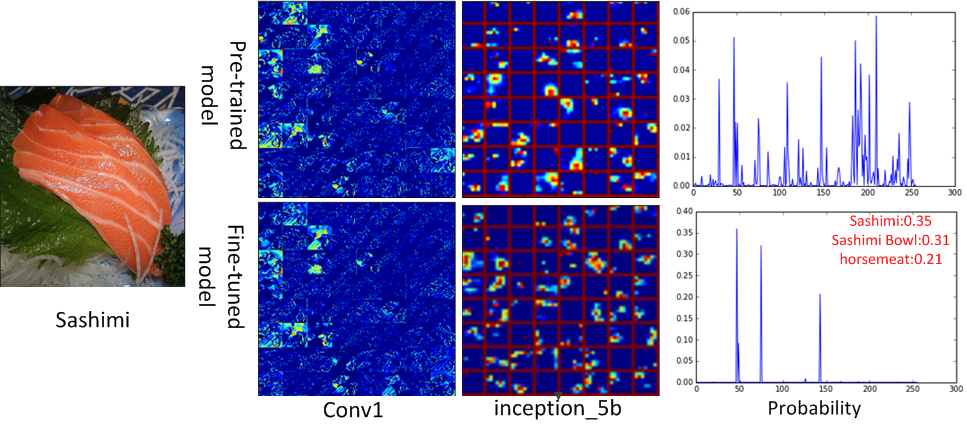
\includegraphics[scale=0.5]{fig/sashimi.png}\\
  \caption{Visualization of some feature maps of different GoogLeNet models in different layers for the same input image. 64 feature maps of each layer are shown. Conv1 is the first convolutional layer and Inception\_5b is the last convolutional layer. }
   \label{fig:sashimi}
\end{figure*}
From Table \ref{tab:ft} we can see that fine-tuning the whole network can improve the performance of the CNN for our task. Compared to other traditional computer vision methods (see Table \ref{tab:256} and \ref{tab:101}), GoogLeNet outperforms the other methods with large margins and we provide the state-of-the-art performance of these two food image datasets.

In Figure \ref{fig:sashimi} we visualize the feature maps of the pre-trained GoogLeNet model and fined-tuned GoogLeNet model with the same input image for some layers. We can see that the feature maps of the lower layer are similar as the lower level features are similar for most recognition tasks.
Then we can see that the feature maps in the high-level are different which leads to totally different recognition results.
Since only the last layer (auxiliary classifier) of the ft-last model is optimized, we can infer that the higher level features are more important which is consistent with our intuition. Also from Table \ref{tab:ft}, it is interesting to see that for the Food-101 task, the accuracy of  the scratch models outperforms the pre-trained models. Since Food-101 is a relatively large dataset with 750 images per class while Food-256 dataset is an imbalanced small one, this indicates that it is difficult to obtain a good deep CNN model while the data is insufficient.

From Table \ref{tab:ft} we can see that GoogLeNet always performances better than AlexNet on both datasets. This implies that the higher level features of GoogLeNet are more discriminative compared to AlexNet and this is due to the special architecture of its basic unit, Inception module. Table \ref{tab:cosg} and \ref{tab:cosa} show the weights' cosine similarity of each layer between the fine-tuned models and their pre-trained models. From the results we can see that the weights in the low layer are more similar which implies that these two architectures can learn the hierarchical features. As the low level features are similar for most of the tasks, the difference of the objects is determined by high-level ones which are the combination of these low level features. Also from Table \ref{tab:cosa}, we can observe that, the weights of the pre-trained and fine-tuned models are extremely similar in AlexNet . This can be caused by the size of receptive filed. Since ReLUs are used in both architectures, vanishing gradients do not exist. Rectified activation function is mathematically given by:
      \begin{equation}\label{relu}
        h = \max ({w^T}x,0) = \left\{ {\begin{array}{*{20}{c}}
{{w^T}x}&{{w^T}x > 0}\\
0&{else}
\end{array}} \right.
      \end{equation}

    The ReLU is inactivated when its input is below 0 and its partial derivative is 0 as well. Sparsity can improve the performance of the linear classifier on top, but on the other hand, sparse representations make the network more difficult to train as well as fine-tune. The derivative of the filter is $\frac{{\partial J}}{{\partial w}} = \frac{{\partial J}}{{\partial y}}\frac{{\partial y}}{{\partial w}} = \frac{{\partial J}}{{\partial y}}*x$ where $\frac{{\partial J}}{{\partial y}}$ denotes the partial derivative of the activation function, $y=w^Tx$ and $x$ denotes the inputs of the layer. The sparse input could lead to sparse filter derivative for back propagation which would eventually prevent the errors passing down effectively. Therefore, the filters of the fine-tuned AlexNet is extremely similar. Compared to large receptive field used in AlexNet, the inception module in GoogLeNet employs 2 additional $n\times n\_reduced$ convolutional layers before the $3\times 3$ and $5\times 5$ convolutional layers (see Figure \ref{incept}). Even though the original purpose of these two $1\times 1$ convolutional layer is for computational efficiency, these 2 convolutional layers tend to squeeze their sparse inputs and generate a dense outputs for the following layer. We can see from Table \ref{tab:sparse} that the sparsity of the $n\times n\_reduce$ layers are denser than other layers within the inception module. This makes the filters in the following layer more easily to be trained for transfer learning and generate efficient sparse representations.
  %\item The pooling strategy. In AlexNet, max pooling is applied to all the pooling layers between several convolution layers. During back propagation, the max pooling layer always passes the error to the place where it came from. Since it only came from one place of the receptive field, the back propagation error is sparse and keeps the most filters unchanged. In GoogLeNet, even though, there is a max pooling layer within every inception module, there are other 3 back propagation errors, from $5\times 5\_reduce$ and $3\times 3\_reduce$ that can parse dense back propagation errors to the previous inception module.


\begin{table*}[htbp]
  \centering
  \caption{Cosine similarity of the layers in inception modules between fine-tuned models and pre-trained model for GoogLeNet}
    \begin{tabular}{r|cccccc}
    \toprule
    \multicolumn{7}{c}{food256} \\
    \midrule
          & \multicolumn{1}{l}{1x1} & \multicolumn{1}{l}{3x3\_reduce} & \multicolumn{1}{l}{3x3} & \multicolumn{1}{l}{5x5\_reduce} & \multicolumn{1}{l}{5x5} & \multicolumn{1}{l}{pool\_proj } \\
    inception\_3a & 0.72  & 0.72  & 0.64  & 0.67  & 0.73  & 0.69 \\
    inception\_3b & 0.59  & 0.64  & 0.53  & 0.70  & 0.60  & 0.56 \\
    inception\_4a & 0.46  & 0.53  & 0.54  & 0.50  & 0.67  & 0.38 \\
    inception\_4b & 0.55  & 0.58  & 0.63  & 0.52  & 0.69  & 0.41 \\
    inception\_4c & 0.63  & 0.64  & 0.63  & 0.57  & 0.68  & 0.52 \\
    inception\_4d & 0.60  & 0.62  & 0.60  & 0.58  & 0.68  & 0.50 \\
    inception\_4e & 0.60  & 0.61  & 0.67  & 0.61  & 0.68  & 0.50 \\
    inception\_5a & 0.51  & 0.53  & 0.58  & 0.48  & 0.60  & 0.39 \\
    inception\_5b & 0.40  & 0.44  & 0.50  & 0.41  & 0.59  & 0.40 \\  \toprule
    \multicolumn{7}{c}{food101} \\ \midrule
          & \multicolumn{1}{l}{1x1 } & \multicolumn{1}{l}{3x3\_reduce} & \multicolumn{1}{l}{3x3} & \multicolumn{1}{l}{5x5\_reduce} & \multicolumn{1}{l}{5x5} & \multicolumn{1}{l}{pool\_proj } \\
    inception\_3a & 0.71  & 0.72  & 0.63  & 0.67  & 0.73  & 0.68 \\
    inception\_3b & 0.56  & 0.63  & 0.50  & 0.71  & 0.60  & 0.53 \\
    inception\_4a & 0.43  & 0.50  & 0.50  & 0.47  & 0.62  & 0.36 \\
    inception\_4b & 0.48  & 0.52  & 0.57  & 0.50  & 0.67  & 0.35 \\
    inception\_4c & 0.57  & 0.61  & 0.59  & 0.53  & 0.63  & 0.47 \\
    inception\_4d & 0.54  & 0.58  & 0.53  & 0.54  & 0.64  & 0.44 \\
    inception\_4e & 0.53  & 0.54  & 0.61  & 0.55  & 0.62  & 0.42 \\
    inception\_5a & 0.43  & 0.47  & 0.53  & 0.45  & 0.57  & 0.34 \\
    inception\_5b & 0.36  & 0.39  & 0.46  & 0.38  & 0.52  & 0.37 \\
    \bottomrule
    \end{tabular}%
  \label{tab:cosg}%
\end{table*}%


\begin{table*}[htbp]
  \centering
  \caption{Cosine similarity of the layers between fine-tuned models and pre-trained model for AlexNet}
    \begin{tabular}{r|ccccccc}
    \toprule
          & conv1 & conv2 & conv3 & conv4 & conv5 & fc6   & fc7 \\
    \midrule
    food256 & 0.997 & 0.987 & 0.976 & 0.976 & 0.978 & 0.936 & 0.923 \\
    food101 & 0.996 & 0.984 & 0.963 & 0.960 & 0.963 & 0.925 & 0.933 \\
    \bottomrule
    \end{tabular}%
  \label{tab:cosa}%
\end{table*}%

% Table generated by Excel2LaTeX from sheet 'google'
\begin{table*}[htbp]
  \centering
  \caption{Sparsity of the output for each unit in GoogLeNet inception module for training data from Food101 in percent}
    \begin{tabular}{r|cccccc}
    \toprule
          & 1x1  & 3x3\_reduce & 3x3  & 5x5\_reduce & 5x5  & pool\_proj  \\
    \midrule
    inception\_3a & $69.3\pm 1.3$  & $69.6 \pm 1.1$  & $80.0\pm  1.0$& $64.1\pm  2.2$& $75.8\pm  1.6$& $76.2\pm 5.4$\\
    inception\_3b & $92.8 \pm 0.9$&$ 76.5 \pm 0.9$& $94.7\pm 0.9 $&$ 71.6 \pm 2.3 $&$ 94.4\pm 0.5 $&$ 94.7 \pm 1.6$\\
    inception\_4a & $90.9 \pm 0.9$& $70.0\pm 1.2 $& $93.8\pm 1.1 $& $63.3\pm 4.0 $& $91.9\pm 1.8 $& $95.1\pm 2.0$\\
    inception\_4b & $71.9 \pm 1.6$& $67.5\pm 1.2$ & $75.4\pm  1.0$& $58.5 \pm 2.6$& $78.9\pm  1.6$& $85.6\pm 3.6$\\
    inception\_4c & $75.1 \pm 2.4$& $72.6 \pm 1.3$& $81.0\pm 2.0$ & $66.3\pm 6.1 $& $79.7 \pm 3.6$& $88.1\pm 3.3$\\
    inception\_4d & $87.3 \pm 2.7$& $78.0 \pm 2.2$& $88.0\pm 1.6$& $67.9\pm 3.1 $& $88.9\pm 2.8 $& $93.0\pm 2.2$\\
    inception\_4e & $91.8\pm  1.1$& $62.3\pm 2.2 $& $91.0\pm 2.5 $& $49.5 \pm 3.7$& $94.0 \pm 1.0$& $92.3\pm 1.5$\\
    inception\_5a & $78.7 \pm 1.6$& $66.5\pm  1.7$& $82.3\pm 2.6 $& $59.9\pm 3.2 $& $86.4\pm 2.3 $& $87.1\pm 2.6$\\
    inception\_5b & $88.2\pm 2.3 $& $86.8 \pm 1.6$&$ 83.3\pm 4.4$ & $84.0\pm 3.1 $& $81.4\pm 5.3$  & $94.7\pm 1.5$\\
    \bottomrule
    \end{tabular}%
  \label{tab:sparse}%
\end{table*}%

The unique structure of the Inception module guarantees that the sparse outputs from previous layer can be squeezed with the $1\times 1$ convolutional layers and feed to convolutional layers with bigger receptive field to generate sparser representation. The squeeze action promises the back propagation error can be transferred more efficiently and makes the whole network more flexible to fit different recogntion tasks.

\subsection{Learning across the datasets}
From the previous experiments we can see that pre-training on the ImageNet dataset can improve the performance of the deep convolutional neural network on our specific area. In this part, we will discuss the generalization ability within the food recognition problem.  Zhou et al. trained AlexNet for Scene Recognition across two datasets with identical categories \cite{NIPS2014_Zhou}. But for more complex situation, such as two similar datasets with a little overlapped categories, we are very interested in exploring whether deep CNN can still successfully handle. Therefore, we conduct the following experiment to stimulate a more challenging real world problem: transferring the knowledge from the fine-tuned Food-101 model to a target set, Food-256 dataset. To make the experiment more practical, we limit the number of samples per category from Food-256 for training, because if we want to build a our own model using deep CNN for a specific task, the resource is always limited and it is exhausted to collect hundreds of labeled images for each category.

The Food-101 and Food-256 datasets share about 46 categories of food even though the images in the same category may vary across these two datasets. The types of food in Food-101 are mainly western style while most types of food in Food-256 are typical Asian foods. We compare the top-5 accuracy trained from different size of subset for Food-256 on different pre-trained model and the results are shown in Table \ref{tab:cross}.
%The ImageNet columns denote  the pre-trained model trained only on ImageNet images and the Food101\_ft columns denote the pre-trained model trained on ImageNet images and then fine-tuned on Food-101.
The ImageNet columns denote using the model pre-trained from ImageNet dataset as the pre-trained model and Food101\_ft columns denote using the fine-tuned Food-101 model (the same one in Table \ref{tab:ft}) as the pre-trained model.

From the result of Table \ref{tab:cross} we can see that, with this further transfer learning, both CNNs can achieve around 95\% of the accuracy trained on full dataset while just utilizing about half of them (50 per class, 12800 of 25361 images). This indicates that when there is not enough labeled data, with its strong generalization ability, deep CNN trained from general task can still achieve satisfying result and perform even better when an additional relevant dataset is involved. This encouraging result may attract more people to use deep CNN for their specific task and continue to explore the potential of the existing architecture as well as designing new ones.

\begin{table*}[htbp]
  \centering
  \caption{Top5 Accuracy for transferring from Food101 to subset of Food256 in percent}
    \begin{tabular}{c|cc|cc}
    \toprule
          & \multicolumn{2}{c|}{AlexNet} & \multicolumn{2}{c}{GoogLeNet} \\
    \midrule
    instances per class & ImageNet  & Food101\_ft    &  ImageNet  & Food101\_ft \\ \midrule
    20    & 68.80  & {75.12} & 74.54 & {77.77} \\
    30    & 73.15 & {77.02} & 79.21 & {81.06} \\
    40    & 76.04 & {80.23} & 81.76 & {83.52} \\
    50    & 78.90  & {81.66} & 84.22 & {85.84} \\
    all    & 85.59 &  {87.21} & {90.66 }&   {90.65}     \\
    \bottomrule
    \end{tabular}%
  \label{tab:cross}%
\end{table*}%


\section{Warm Start Domain Adaptation for Learning New Categories}\label{sec:da}
For a real world recognition task, an algorithm that can continuously adaptive to new labels just like the human does, is always very attractive and practical.
In this section, we propose an adaptive method for learning new categories with a few target examples using the feature representations from GoogLeNet. By warm start the parameters of the classifiers, our method can effectively learning new categories. The experiment results show that our method is able to adapt new categories with just a few examples and outperforms the method that learning directly with a large margin.
For the rest part of this section, we first discuss the limitation of some previous domain adaptation approaches for our task, then we introduce our method and show the improved performance on the same task.

%To illustrate our method, we design the following experiment, transferring from Food-101 dataset to Food-256 dataset while just using a few examples. Since Food-101 has more images per category, we use it as the source domain and the fine-tuned GoogLeNet on Food-101 from Section \ref{sec:ft} is used as the feature extractor to generate feature representations for both datasets.
%
%Food-101 and Food-256 datasets share about 36 categories even though the images in the same category may vary across these two datasets. The types of food in Food-101 are mainly western style while most types of food in Food-256 are typical Asian foods. To make this task more challenging, we also limited the number of examples in both source and target domain. Unlike those previous studies which only consider the performance within the target domain, since the two domains are within the general food domain, we combine these two domains together as a more general super-domain and evaluate the accuracy over all the categories in this super-domain.
%The experiment results show our method is able to adapt new categories and outperforms the method that learning directly with a large margin.
%For the rest part of this section, we first discuss the limitation of some previous domain adaptation approaches for our task, then we introduce our method and show the improved performance on the same task.
\subsection{Limits of previous approaches}
From previous studies, there are two kinds of approach to solve our task. The first approach is to fine-tuning the deep CNN with the target examples incorporating with the sources ones.
Fine-tuning the deep CNN model focuses on learning good feature representations from the images and using linear models for classification. From Section \ref{sec:ft}, we successfully use this approach to transfer the knowledge from a general domain to our food domain with impressive results. Indeed, deep CNN can learn discriminative features effectively and by taking advantage of this, this approach achieved some impressive results from previous studies\cite{Chatfield14} \cite{zeiler2014visualizing}. However, fine-tuning on deep CNN requires an ample amount of labeled target data and sometimes could degrade the performance when the labeled examples are scarce\cite{hoffman2013one}. There are many hyperparameters that affect the performance of deep CNN and fine-tuning it on a sparse label condition can lead to horrible overfitting. Apart from its sensitivity to the hyperparameters, fine-tuning the whole network requires intensive computational resources which makes it inappropriate for online learning.

Rather than learning efficient representations, another typical approach are more focused on dealing with the representation learned from conventional feature extraction methods for domain adaptation.
%Many methods have been proposed by minimizing the representation distance between the source and target domain in an unsupervised manner \cite{gong2012geodesic}\cite{fernando2013unsupervised}.
Supervised domain adaptation models, such as Adaptive-SVM (A-SVM) and PMT-SVM, try to utilize the knowledge from source domain and apply to target domain and hypothesize that there should be a relatively strong relationship between the categories among these two domains\cite{yang2007adapting}\cite{aytar2011tabula}. These methods are limited in our task for the reasons that all these methods try to find the similarity between the source and target domain. Indeed, they work well when these two domains have many overlapped or similar categories. However, sparse representations from deep CNN from which the linear classifiers would eventually benefit indicates that the distance of the representations between different categories could be very large.

From empirical experiments, we find that adaptive methods suffer as the difference of source and target categories increases. Table \ref{tab:su_domian} shows some empirical experiment results for two typical domain adaptation methods in a binary classification scenario. We manually choose the similar/identical source categories for the target ones if possible. For the those categories which we fail to find even similar category in source domain, we just choose the category whose representations are most similar to the target one measured by cosine similarity. The parameters used in these methods are set as the default because we think that tuned the parameters for these methods won't improve the performance very much for this experiment.  From the result of our simple experiment, we can see that A-SVM and PMT-SVM suffers from choosing the appropriate domain categories for new categories in target domain. And for our task which is a multi-class situation and more complicated than this, the performance of these methods could be worse than training without any of these adaptive methods.
% Table generated by Excel2LaTeX from sheet 'Sheet1'
\begin{table*}[htbp]
  \centering
  \caption{Average Precision for A-SVM, PMT-SVM, SVM and Logistic Regression. Source categories without * are determined by cosine similarity}
    \begin{tabular}{cccccc}
    \toprule
    Category from food 256 & Category from food 101 & A-SVM  & PMT-SVM & SVM &LR\\
    \midrule
%    Green salad & Caesar salad & 0.1627 & 0.1622 \\
    Doughnut & Doughnut & 0.4771 & 0.4735 &0.4781&0.4554\\
    Caesar salad &  Caesar salad & 0.9488 & 0.9496 &0.9498&0.9486\\
    White rice  & Fried rice & 0.8118 & 0.7932 &0.7932&0.9004\\
    Oatmeal & French onion soup* & 0.0345 & 0.0381 & 0.0347 &0.0454\\
    Pork cutlet & French fries* & 0.0446 & 0.0381 &0.0450& 0.0837\\
    \bottomrule
    \end{tabular}%
  \label{tab:su_domian}%
\end{table*}%

As far as we know, few study has shown that there is an approach that can solve our task.
\subsection{Online adaptive learning for new category}
Chu et al. recently proposed a warm start approach for parameter selection in linear model and by iteratively updating the parameters optimized from previous knowledge, the algorithm can search the optimal value for a specific task\cite{chuwarm}. Inspired by this, we propose a warm start adaptive learning algorithm that can adapt new categories from the target domain in an online learning module. Instead of learning the whole target categories directly, our method adapts one category each time and iteratively updates all the parameters. 
Our method uses logistic regression to classify the representations obtained from deep CNN. 
For the new category in target domain, rather than utilizing the parameters from source domain, we employ another negative binary classifier pre-trained with all the examples from other categories as the negative class and warm start the classifier with the parameters of the negative classifier for the new category. This approach can be extended into an online domain adaptation scenario when the algorithm just adopts one new category in each step for multi-class target domain situation. For each step, considering $M$ categories in the source domain $S$ and a new category $t$ from target domain $T$, there are $M$ binary classifiers $F=\left\{ {{f}\left( {{w_i},{b_i}} \right)} \right\}_{i = 1}^M$ for each category in $S$ and the negative classifier $\hat{f}=f(\hat{w},\hat{b})$ using all the examples in $\mathcal{P^-}=S$ as negative examples. The classifier $f_t$ for the new category $t$ is initialized with $\left\{\hat{w},\hat{b}\right\}$ and trained with $\mathcal{P^-}\bigcup\mathcal{P^+}$ while $\mathcal{P^+}=t$. Then we update the negative classifier $\hat{f}$ with negative examples $\mathcal{P^-}=S\bigcup t$. The complete strategy for our method is given in Algorithm \ref{algo:ws}.
\begin{algorithm}
  \caption{Complete algorithm of warm start adaptation}\label{algo:ws}
  \begin{algorithmic}[1]
    \REQUIRE Source domain $S = \{ {s_i}|i = 1,..M\} $, Target domain $T = \{ {t_j}|j = 1,..N\} $, Classifier $F = \{\emptyset\}$
    \ENSURE $F$\\
    \FORALL {$i\in M$}
         \STATE $\mathcal{P^+}\leftarrow s_i, \mathcal{P^-}\leftarrow S-s_i$\\
          Train ${{f_i}\left( {{w_i},{b_i}} \right)}$ with $\mathcal{P^+}\bigcup\mathcal{P^-}$, $F\leftarrow F\bigcup f_i$
    \ENDFOR
    \STATE Training negative $\hat{f}\left( {\hat{w_i},\hat{b_i}} \right)$ with $\mathcal{P^-}=S$
    \WHILE {$t_j  \notin S$}
         \FORALL {$i\in M$}
             \STATE $\mathcal{P^+}\leftarrow s_i, \mathcal{P^-}\leftarrow S-s_i+t_j$ \\
              Update ${{f_i}\left( {{w_i},{b_i}} \right)}$ with $\mathcal{P^+}\bigcup\mathcal{P^-}$
        \ENDFOR
        \STATE Initialize $f_j$ with $(\hat{w},\hat{b})$ and train with .
        \STATE $F\leftarrow\ F\bigcup f_j$
        \STATE $S\leftarrow S\bigcup t_j, M\leftarrow M+1$
        \STATE Update $\hat{f}$ with $\mathcal{P^-}=S+t_j$
     \ENDWHILE
  \end{algorithmic}
\end{algorithm}
In our task, compared to those methods using the previous parameters directly, the warm start can start with a better initialization for the new category and thus can be more adaptive for new categories. We use Stochastic Gradient Descent (SGD) to update the parameters for all the binary classifiers as well as the negative classifier.
\begin{figure*}
  \centering
  % Requires \usepackage{graphicx}
  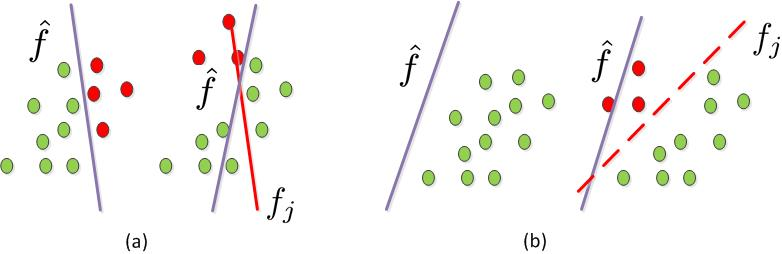
\includegraphics[scale = .6]{fig/domain.jpg}\\
  \caption{(a) Conventional adaptation method fail to find good initialization for the new category from source domain. (b) The parameters from $\hat{f}$ are more adaptive for the new categories.}
  \label{fig:wm}
\end{figure*}

\subsection{Experiment setup \& Evaluation}
To illustrate our method, we design the following experiment, transferring from Food-101 dataset to Food-256 dataset while just using a few examples. Since Food-101 has more images per category, we use it as the source domain and the fine-tuned GoogLeNet on Food-101 from Section \ref{sec:ft} is used as the feature extractor to generate feature representations for both datasets and deep feature representations from \emph{Pool5}, the layer before auxiliary linear classifier, are used as the inputs of our method.

The types of food in Food-101 are mainly western style while most types of food in Food-256 are typical Asian foods. They share about 36 categories even though the images in the same category may vary across these two datasets. These 36 duplicated categories are removed as noisy categories, so there are 220 new categories left in Food-256 dataset.
To make this task more challenging, we also limited the number of examples in both source and target domain.

Baseline: Instead of using the supervised adaptation techniques, such as A-SVM, we use cold start which randomly initializes the parameters for all the classifiers, as our baseline, because from Table \ref{tab:su_domian} we can see when adapting new categories, SVM and LR without any adaptation technique show similar results to those adaptive methods. The hypothesis of these adaptive methods limits their ability to adapt new categories as we discuss above.

\emph{n shorts:} In our experiments, the training set of $n$ shots contains $n$ randomly picked examples from each category in both Food-101 and Food-256 datasets and the test set contains all the rest examples in Food-256 only.

For our SGD, we use effective learn rate following polynomial decay, to be 0 at max iteration and set base learning rate to 0.01. The initialization of the classifiers for source domain are trained with all the examples from source domain and negative classifier are initialized the same way as well. Unlike the other studies which consider the performance within the target domain separately, since the categories in our two datasets are in the general food category we would rather considering to combine them together as a super-domain and evaluate the performance for target categories on this super-domain.
\subsection{From 101 to 102 categories}
When there are multiple categories in target domain, our method divides the learning procedure into several steps and adapts one category in each step, updating all the parameters of the binary logistic regression classifiers. So for the experiment adapting Food-256 from Food-101, the algorithm starts from a 101 to 102 categories situation. We conduct the following experiment: we try to add an arbitrary category from Food-256 to Food-101 and evaluate accuracy of the new category in the super-domain containing 102 categories. We go through all the 220 categories in Food-256 in each round and Table \ref{tab:N+1} shows the average performance of 10 rounds experiments.

\begin{table}[htbp]
  \centering
  \caption{Accuracy for a single new target category in M+1 experiment. Average top-5 accuracies for some categories are shown. Last row shows the average results for all categories.}
    \begin{tabular}{c|cc|cc}
    \toprule
          & \multicolumn{2}{c|}{5 shots} & \multicolumn{2}{c}{1 shot} \\
    \midrule
       target category   & \multicolumn{1}{c}{Warm} & \multicolumn{1}{c|}{Cold} & \multicolumn{1}{c}{Warm} & \multicolumn{1}{c}{Cold} \\
        \midrule
    crape & \textbf{84.16} & 62.29 & \textbf{56.20}  & 28.00 \\
   chip butty & \textbf{80.97} & 65.82 & \textbf{55.03} & 37.40 \\
    meat loaf & \textbf{67.78} & 53.15 & \textbf{68.21} & 56.07 \\
    dried fish & \textbf{92.00}    & 79.81 &\textbf{83.85} & 71.19 \\
   scrambled egg & \textbf{75.21} & 63.54 & \textbf{59.00}    & 43.20 \\
    pork belly & \textbf{81.76 }& 70.59 &\textbf{53.21} & 32.45 \\
%    natto & 79.01&\textbf{80.70}&\textbf{73.69}&66.71\\
%    miso soup &\textbf{96.06}&95.92&91.04&\textbf{94.52}\\
    \midrule
    %Average &\textbf{91.91$\pm$8.15}&88.82$\pm$10.40  & \textbf{80.77$\pm$ 12.03} & $71.78\pm 15.07 $ \\
    Overall average &\textbf{91.91}&88.82  & \textbf{80.77} & 71.78 \\
    \bottomrule
    \end{tabular}%
  \label{tab:N+1}%
\end{table}%
From Table \ref{tab:N+1} we can see that by taking advantage of the warm start, the warm start does a slightly better than cold start in M+1 experiment since the initialization difference between these two methods are too small. We believe the margin of these two methods would increase as more new categories are learned from warm start.
%%%%%%%%%%%%%%%%%%%%%%%%%%%%%%%%%%%%%%%%%%%%%%%%%%%%%%%%%%%%%%%%%%%

\subsection{From 101 to 101+220 categories}
In this part, we show the performance of warm start in multiple new categories situation. From the experiments above, warm start shows some improvement on cold start and experiment shows that the improvement can be accumulated as more categories are learned. Because the parameters of the negative classifier can affect the whole procedure greatly and randomly picking only one example from each category can be significantly bias, we fail to get a convergent result for both warm and cold starts in one short experiment.
From empirical experiments we find that in order to get a convergent result, we have to pick at least 5 examples in each category. So we only show the performance of five shots for this experiment. In each step, the new category is determined by its original class index in Food-256. We use run SGD 50 iterations for each step and run this experiment 10 times as well. Figure \ref{fig:wama} shows the average results in 5 short for both warm and cold start in each step.

\begin{figure*}
  \centering
    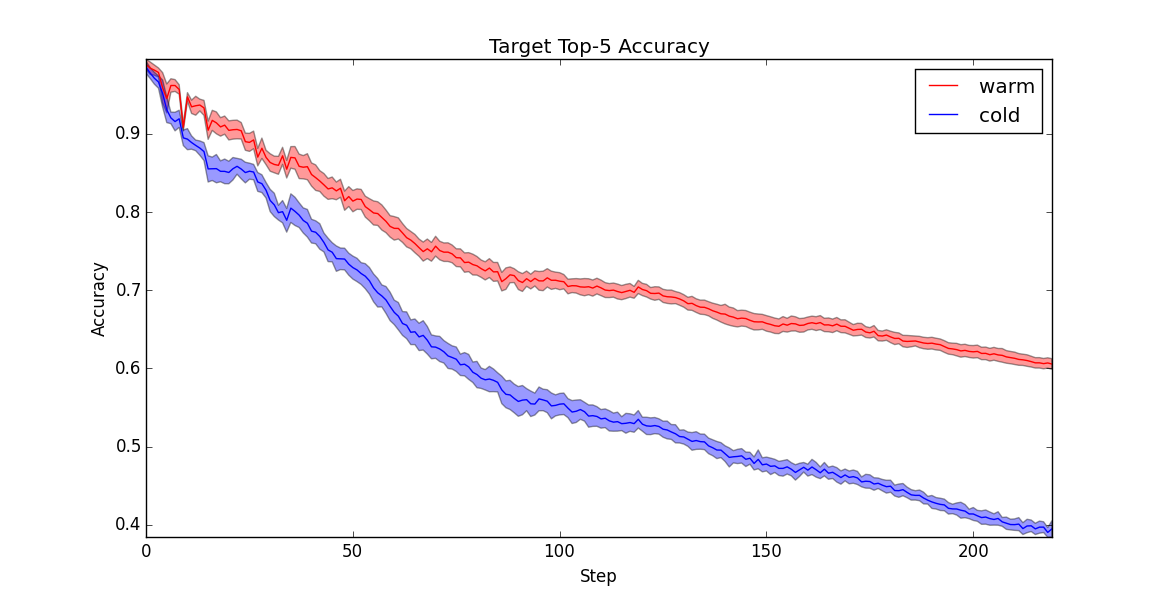
\includegraphics[scale=0.4]{fig/M+N.png}
    \caption{Top-5 accuracy curve for categories in Food-256 in super-domain with 5 shots. Mean and standard deviation are shown.}
      \label{fig:wama}
\end{figure*}

From Figure \ref{fig:wama} we can see that benefitting from warm start, classifiers can accumulate the information from previous steps and thus the margin between warm and cold starts increases as more new categories are learned. Indeed, cold start may not converge well for just 50 iterations. We believe that given enough training iteration, warm start can still converge to a better result (see Figure \ref{fig:errdiff}). We compare the results for different iterations and the average performance of 10 experiments are shown in Table \ref{tab:it}. The result of cold start in 20 iterations experiments are ignored because it shows similar result to random guess. We observe that increasing training iteration won't help improve the performance of warm start very much as it converges very fast by taking advantage of better initialization.
\begin{figure*}[htbp]
\centering
\subfigure{
    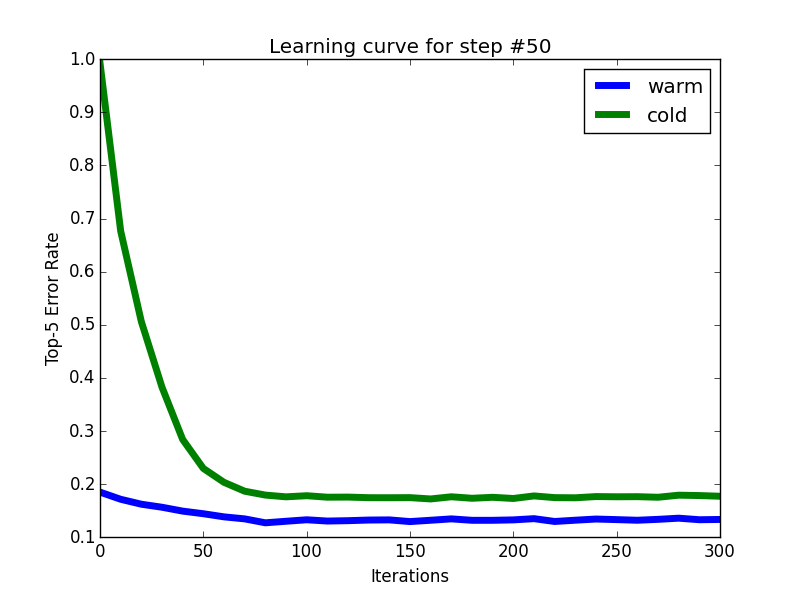
\includegraphics[width=0.3\textwidth]{fig/50W.png}
}
\subfigure{
    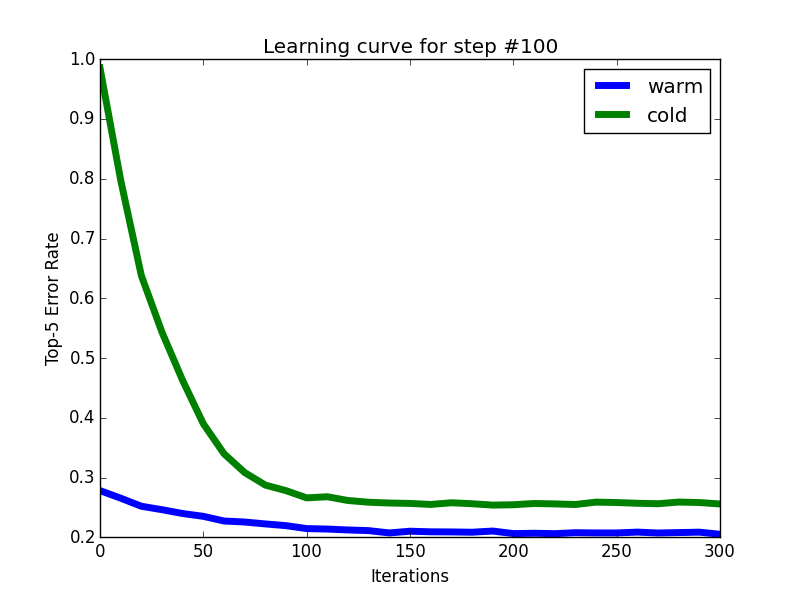
\includegraphics[width=0.3\textwidth]{fig/100W.png}
}\\
\subfigure{
    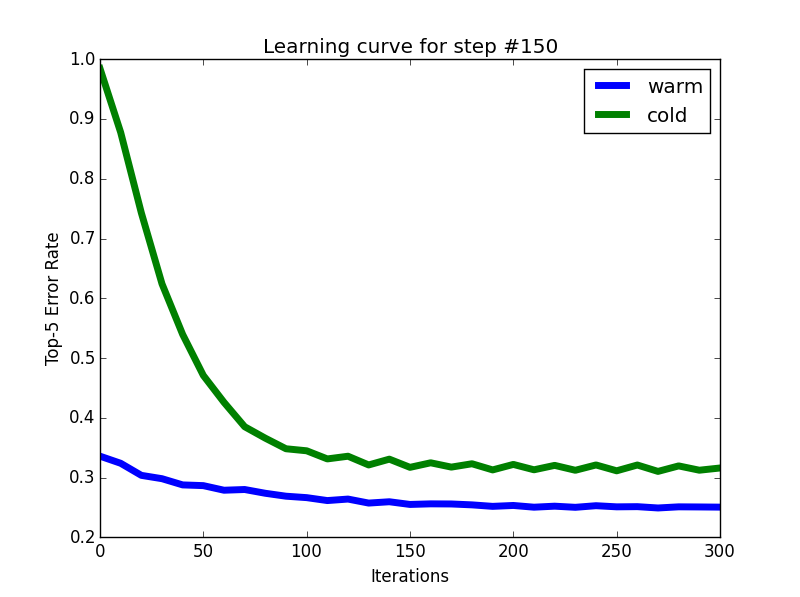
\includegraphics[width=0.3\textwidth]{fig/150W.png}
}
\subfigure{
    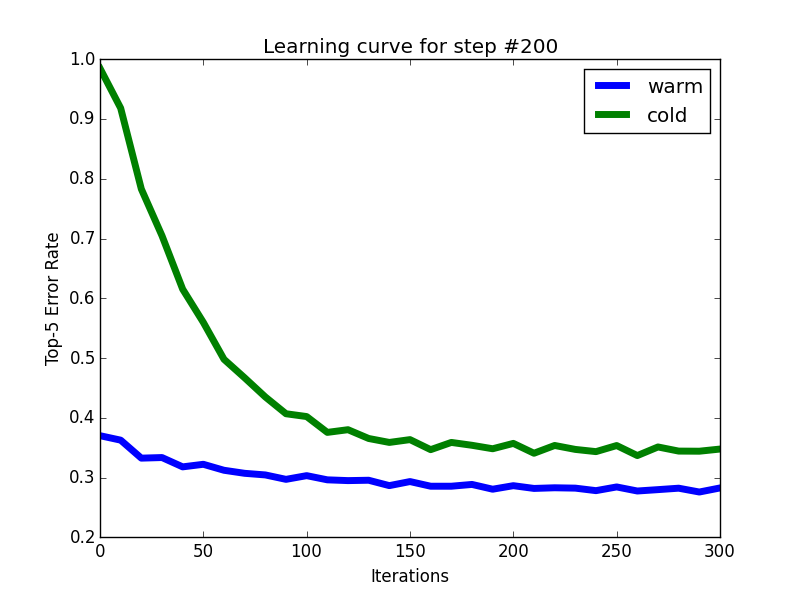
\includegraphics[width=0.3\textwidth]{fig/200W.png}
}
\caption{Overall learning curve in some steps for 300 iterations. \textbf{Observation:} training with enough iteration, warm start can still outperforms cold start in a single step.}
\label{fig:errdiff}
\end{figure*}
% Table generated by Excel2LaTeX from sheet 'Sheet1'
\begin{table*}[htbp]
  \centering
  \caption{Top-5 accuracy for 220 new categories in super-domain with different training iteration in each step.}
    \begin{tabular}{C{1cm}c|c|cc|cc}
    \toprule
          & 10 iterations&20 iterations &\multicolumn{2}{c|}{50 Iterations} & \multicolumn{2}{c}{300 iterations} \\
    \midrule
          & warm start & warm start& warm start & cold start & warm start & cold start \\
    Top-5& 60.37$\pm$ 0.58&60.54$\pm0.32$  &60.33$\pm$0.62   &     39.10$\pm$0.66   &    \textbf{61.48$\pm$0.59 }  & 55.35$\pm$0.48 \\
    \bottomrule
    \end{tabular}%
  \label{tab:it}%
\end{table*}%

\section{Conclusion}
In this paper, we propose a method that can adapt new categories using warm start parameters and deep feature representations. In order to obtain efficient feature representations, we first train a deep neural network as our feature extractor. Compared to previous shallow methods, our deep CNN model achieves the state-of-the-art performance on Food-101 dataset. Unlike many previous methods that can just adapt identical/similar categories between domains,  our method can iteratively learn new categories. By learning one new category and warm start with the parameters from negative classifier in each step, our method shows improved result compared to training with the examples from new categories directly.

Our method can be a very efficient method when the computational resource is limited, such as mobile device etc. The idea of warm start can achieve a better result with just a few training iterations. Our future work can be a natural extension of this work: learning efficient shallow model from deep representations when the target examples are limited, such as one shot learning etc. In this scenario, randomly pick few examples from each categories could not be the best solution. Sophisticated pooling strategy could be a possible way to best eliminate the bias of data size.



% An example of a floating figure using the graphicx package.
% Note that \label must occur AFTER (or within) \caption.
% For figures, \caption should occur after the \includegraphics.
% Note that IEEEtran v1.7 and later has special internal code that
% is designed to preserve the operation of \label within \caption
% even when the captionsoff option is in effect. However, because
% of issues like this, it may be the safest practice to put all your
% \label just after \caption rather than within \caption{}.
%
% Reminder: the "draftcls" or "draftclsnofoot", not "draft", class
% option should be used if it is desired that the figures are to be
% displayed while in draft mode.
%
%\begin{figure}[!t]
%\centering
%\includegraphics[width=2.5in]{myfigure}
% where an .eps filename suffix will be assumed under latex,
% and a .pdf suffix will be assumed for pdflatex; or what has been declared
% via \DeclareGraphicsExtensions.
%\caption{Simulation Results}
%\label{fig_sim}
%\end{figure}

% Note that IEEE typically puts floats only at the top, even when this
% results in a large percentage of a column being occupied by floats.


% An example of a double column floating figure using two subfigures.
% (The subfig.sty package must be loaded for this to work.)
% The subfigure \label commands are set within each subfloat command, the
% \label for the overall figure must come after \caption.
% \hfil must be used as a separator to get equal spacing.
% The subfigure.sty package works much the same way, except \subfigure is
% used instead of \subfloat.
%
%\begin{figure*}[!t]
%\centerline{\subfloat[Case I]\includegraphics[width=2.5in]{subfigcase1}%
%\label{fig_first_case}}
%\hfil
%\subfloat[Case II]{\includegraphics[width=2.5in]{subfigcase2}%
%\label{fig_second_case}}}
%\caption{Simulation results}
%\label{fig_sim}
%\end{figure*}
%
% Note that often IEEE papers with subfigures do not employ subfigure
% captions (using the optional argument to \subfloat), but instead will
% reference/describe all of them (a), (b), etc., within the main caption.


% An example of a floating table. Note that, for IEEE style tables, the
% \caption command should come BEFORE the table. Table text will default to
% \footnotesize as IEEE normally uses this smaller font for tables.
% The \label must come after \caption as always.
%
%\begin{table}[!t]
%% increase table row spacing, adjust to taste
%\renewcommand{\arraystretch}{1.3}
% if using array.sty, it might be a good idea to tweak the value of
% \extrarowheight as needed to properly center the text within the cells
%\caption{An Example of a Table}
%\label{table_example}
%\centering
%% Some packages, such as MDW tools, offer better commands for making tables
%% than the plain LaTeX2e tabular which is used here.
%\begin{tabular}{|c||c|}
%\hline
%One & Two\\
%\hline
%Three & Four\\
%\hline
%\end{tabular}
%\end{table}


% Note that IEEE does not put floats in the very first column - or typically
% anywhere on the first page for that matter. Also, in-text middle ("here")
% positioning is not used. Most IEEE journals/conferences use top floats
% exclusively. Note that, LaTeX2e, unlike IEEE journals/conferences, places
% footnotes above bottom floats. This can be corrected via the \fnbelowfloat
% command of the stfloats package.








% conference papers do not normally have an appendix


% use section* for acknowledgement
\section*{Acknowledgment}
The authors would like to thank...
%\appendices
%\section{Learning curve for some steps for larger iteration}\label{app:conv}
\begin{figure*}[htbp]
\centering
\subfigure{
    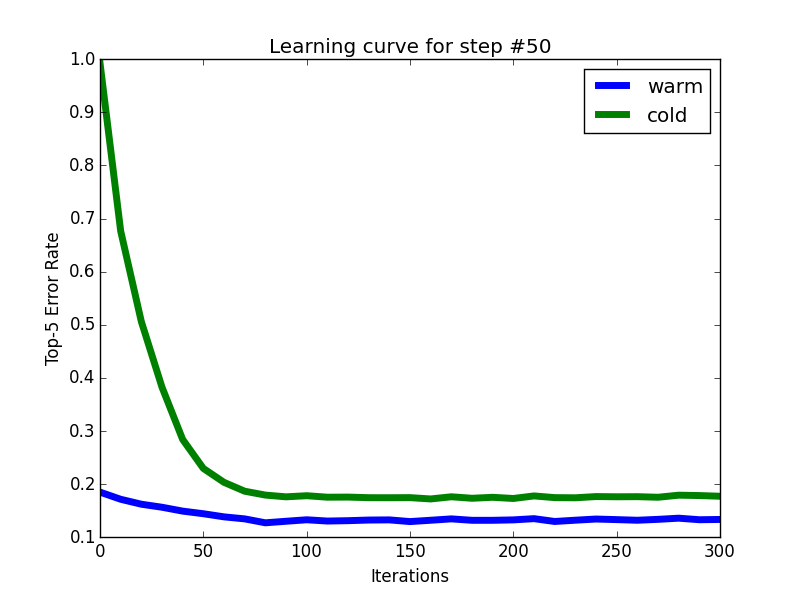
\includegraphics[width=0.4\textwidth]{fig/50W.png}
}
\subfigure{
    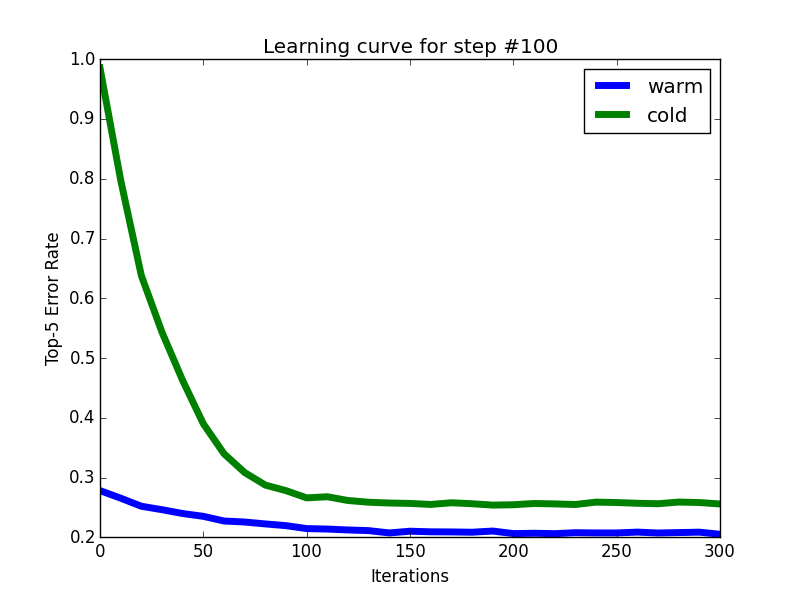
\includegraphics[width=0.4\textwidth]{fig/100W.png}
}\\
\subfigure{
    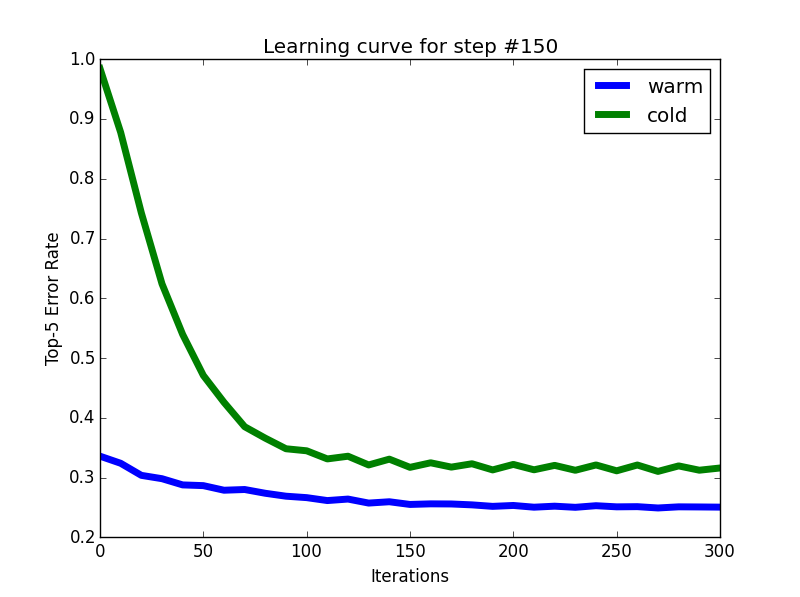
\includegraphics[width=0.4\textwidth]{fig/150W.png}
}
\subfigure{
    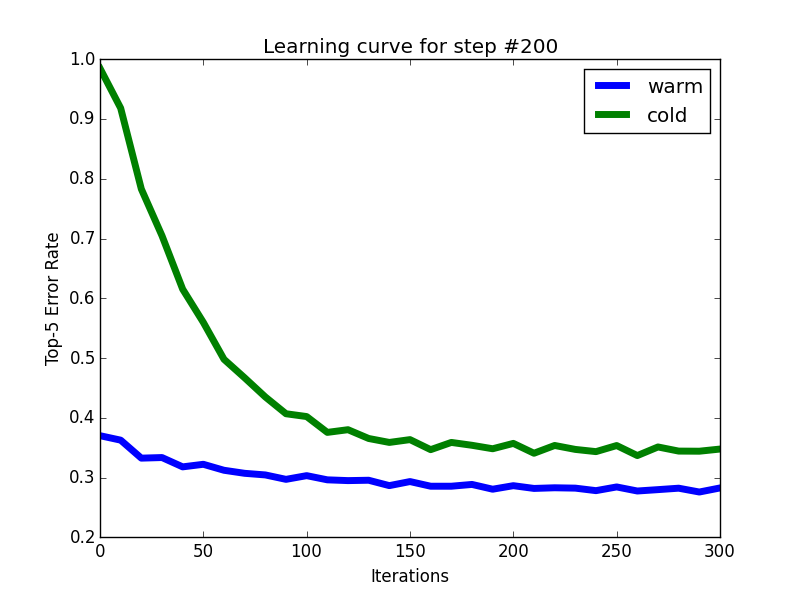
\includegraphics[width=0.4\textwidth]{fig/200W.png}
}
\caption{Overall learning curve in some steps for 300 iterations. Training with enough iterations, warm start can still outperforms cold start.}
\label{fig:errdiff}
\end{figure*}







% trigger a \newpage just before the given reference
% number - used to balance the columns on the last page
% adjust value as needed - may need to be readjusted if
% the document is modified later
%\IEEEtriggeratref{8}
% The "triggered" command can be changed if desired:
%\IEEEtriggercmd{\enlargethispage{-5in}}

% references section

% can use a bibliography generated by BibTeX as a .bbl file
% BibTeX documentation can be easily obtained at:
% http://www.ctan.org/tex-archive/biblio/bibtex/contrib/doc/
% The IEEEtran BibTeX style support page is at:
% http://www.michaelshell.org/tex/ieeetran/bibtex/
%\bibliographystyle{IEEEtran}
% argument is your BibTeX string definitions and bibliography database(s)
%\bibliography{IEEEabrv,../bib/paper}
%
% <OR> manually copy in the resultant .bbl file
% set second argument of \begin to the number of references
% (used to reserve space for the reference number labels box)
\bibliographystyle{IEEEtran}
\bibliography{IEEEabrv,research}




% that's all folks
\end{document}


